\documentclass[a4paper,12pt]{report} 
\usepackage{amsmath} 
\usepackage[a4paper, total={6in, 10in}]{geometry} 
\usepackage{minted} 
\usepackage{overpic} 
\usepackage{subcaption} 
\usepackage{wrapfig} 
\usepackage{graphicx} 
\usepackage[utf8]{inputenc} 
\usepackage[english]{babel} 
\usepackage[utf8]{inputenc} 
\usepackage{lipsum} 
\usepackage{graphicx} 
\usepackage{floatrow} 
\usepackage[dvipsnames]{xcolor} 
\usepackage[table]{xcolor} 
\usepackage{array, hhline} 
\usepackage{siunitx} 
\usepackage{ragged2e} 
\usepackage[demo]{graphicx} 
\usepackage{verbatimbox} 
\usepackage{tikz} 
\definecolor{mycolor}{rgb}{0,0.6,0.5} 
\tikzset{     ultra thick/.style={line width=10pt} } 
 \usepackage{pgfplots}
\usepackage[english]{babel} 
\usepackage[utf8]{inputenc} 
\usepackage{fancyhdr} 
\usepackage{array} 
\usepackage{multirow} 
\usepackage{multicol} 
\usepackage{tabularx} 
\usepackage{tikz} 
\usepackage{circuitikz} 
\usepackage{lipsum} 
\usepackage{titlesec} 
\pagenumbering{arabic} 
\documentclass[11pt]{article} 
\usepackage[margin=1in]{geometry} 
\documentclass{article} 
\usepackage{blindtext} 

 \begin{document} 
 \setcounter{chapter}{1}
\begin{abstract} 
 
In this project, an IoT based smart energy meter was developed to monitor the voltage, current, power and energy consumption with good accuracy in real time environment. We connected an ESP32 microcontroller, energy monitoring sensors, and an LCD to make the device accurate through calibration techniques or averaging of data. The meter reads 0V, 0A, 0W and 0Wh when no load is connected across the meter and gives accurate readings for any load connected across the meter. Also, it is built to forward the same results to Node-RED system via MQTT via (Wi-Fi) for remote monitoring. From this project, we discovered energy monitoring, IoT, and dealing with the accuracy issues.

\end{abstract} 
\pagebreak 
\tableofcontents  
\pagebreak 

\section{Objectives and Introduction}\label{ch:intro}

\subsection{Objectives}
\begin{itemize}
    \item Design a Smart Energy Meter to measure voltage, current, power, and energy consumption accurately.
    \item Enable IoT-based remote monitoring through MQTT and Node-RED over Wi-Fi.
    \item Provide a user-friendly interface via LCD and Node-RED dashboard.
\end{itemize}

\subsection{Introduction}
\subsection{ESP32 Microcontroller}  
The \textbf{ESP32} is a versatile microcontroller with built-in Wi-Fi and Bluetooth capabilities, ideal for IoT applications like the Smart Energy Meter. It features dual-core processing, a clock speed of up to 240 MHz, and multiple GPIO pins, allowing integration with voltage and current sensors for real-time data acquisition. Its ability to connect wirelessly makes it suitable for remote monitoring and control, a key feature of this project.  

\subsubsection{ZMPT101B Voltage Sensor}  
The \textbf{ZMPT101B} is a high-precision AC voltage sensor designed for accurate voltage measurements in energy monitoring systems. Its main specifications include:  
\begin{itemize}  
    \item Measurement Range: 0--250V AC  
    \item Accuracy: $\pm 0.5\%$  
    \item Compact size and high sensitivity, making it suitable for seamless integration with the ESP32.  
\end{itemize}  
In the Smart Energy Meter, the ZMPT101B measures the AC voltage of the connected load, providing accurate voltage readings essential for power calculations.  

\subsubsection{ACS712T Current Sensor}  
The \textbf{ACS712T} is a Hall-effect-based current sensor used to measure AC and DC currents. Key specifications from its datasheet include:  
\begin{itemize}  
    \item Measurement Range: $\pm 5$A, $\pm 20$A, or $\pm 30$A (depending on the variant)  
    \item Sensitivity: 185 mV/A for the 5A version  
    \item Low noise and fast response time for precise current monitoring  
\end{itemize}  
In this project, the ACS712T is used to measure the current flowing through the connected load, which, combined with voltage readings, calculates power and energy consumption.  

\subsubsection{Node-RED and MQTT for IoT Integration}  
\textbf{Node-RED}, paired with the \textbf{MQTT protocol}, enables the Smart Energy Meter to provide remote monitoring capabilities. Node-RED is a flow-based programming tool for IoT integrations, while MQTT ensures lightweight and reliable communication between devices. The ESP32 publishes real-time sensor data to an MQTT broker via Wi-Fi, and the data is visualized and monitored through Node-RED’s user interface. This setup allows the Smart Energy Meter to be accessed remotely, enhancing convenience and usability.  

By integrating these components, the Smart Energy Meter achieves accurate energy monitoring with real-time remote access through IoT technology.  


\section{Equipments and Methodology}\label{ch:intro}
\subsection{Equipment}
\begin{itemize}
    \item ESP32 Microcontroller
    \item ZMPT101B Voltage Sensor
    \item ACS712T Current Sensor
    \item LCD Display
    \item Node-RED
    \item MQTT Broker
    \item Wi-Fi Router/Access Point
    \item Computer/Server
\end{itemize}

\subsection{Methodology}
\begin{itemize}
    \item The Smart Energy Meter system is to measure voltage, current, power, and energy through the ZMPT101B voltage sensor and ACS712T current sensor.
    \item The ESP32 microcontroller is used to acquire the sensor data and to check the received data ready to be sent.
    \item The collected data is broadcasted to an MQTT broker using Wi-Fi to facilitate real-time data sharing.
    \item The results of data processing are displayed in the Node-RED panel, and the main parameters of energy are monitored remotely.
    \item For conveniently monitoring the measured values, an LCD display and Node-RED dashboard are incorporated for the purpose.
    \item The system is tested to ensure accuracy in measurements and reliability in remote monitoring through IoT integration.
\end{itemize}

\section{Results and Discussion}
\subsection{Results}
Following are the results of our project which shows the energy and power consumption at different states of load
\begin{itemize}
    \item When no load is connected to the sensors
    \begin{figure}[H]
        \centering
        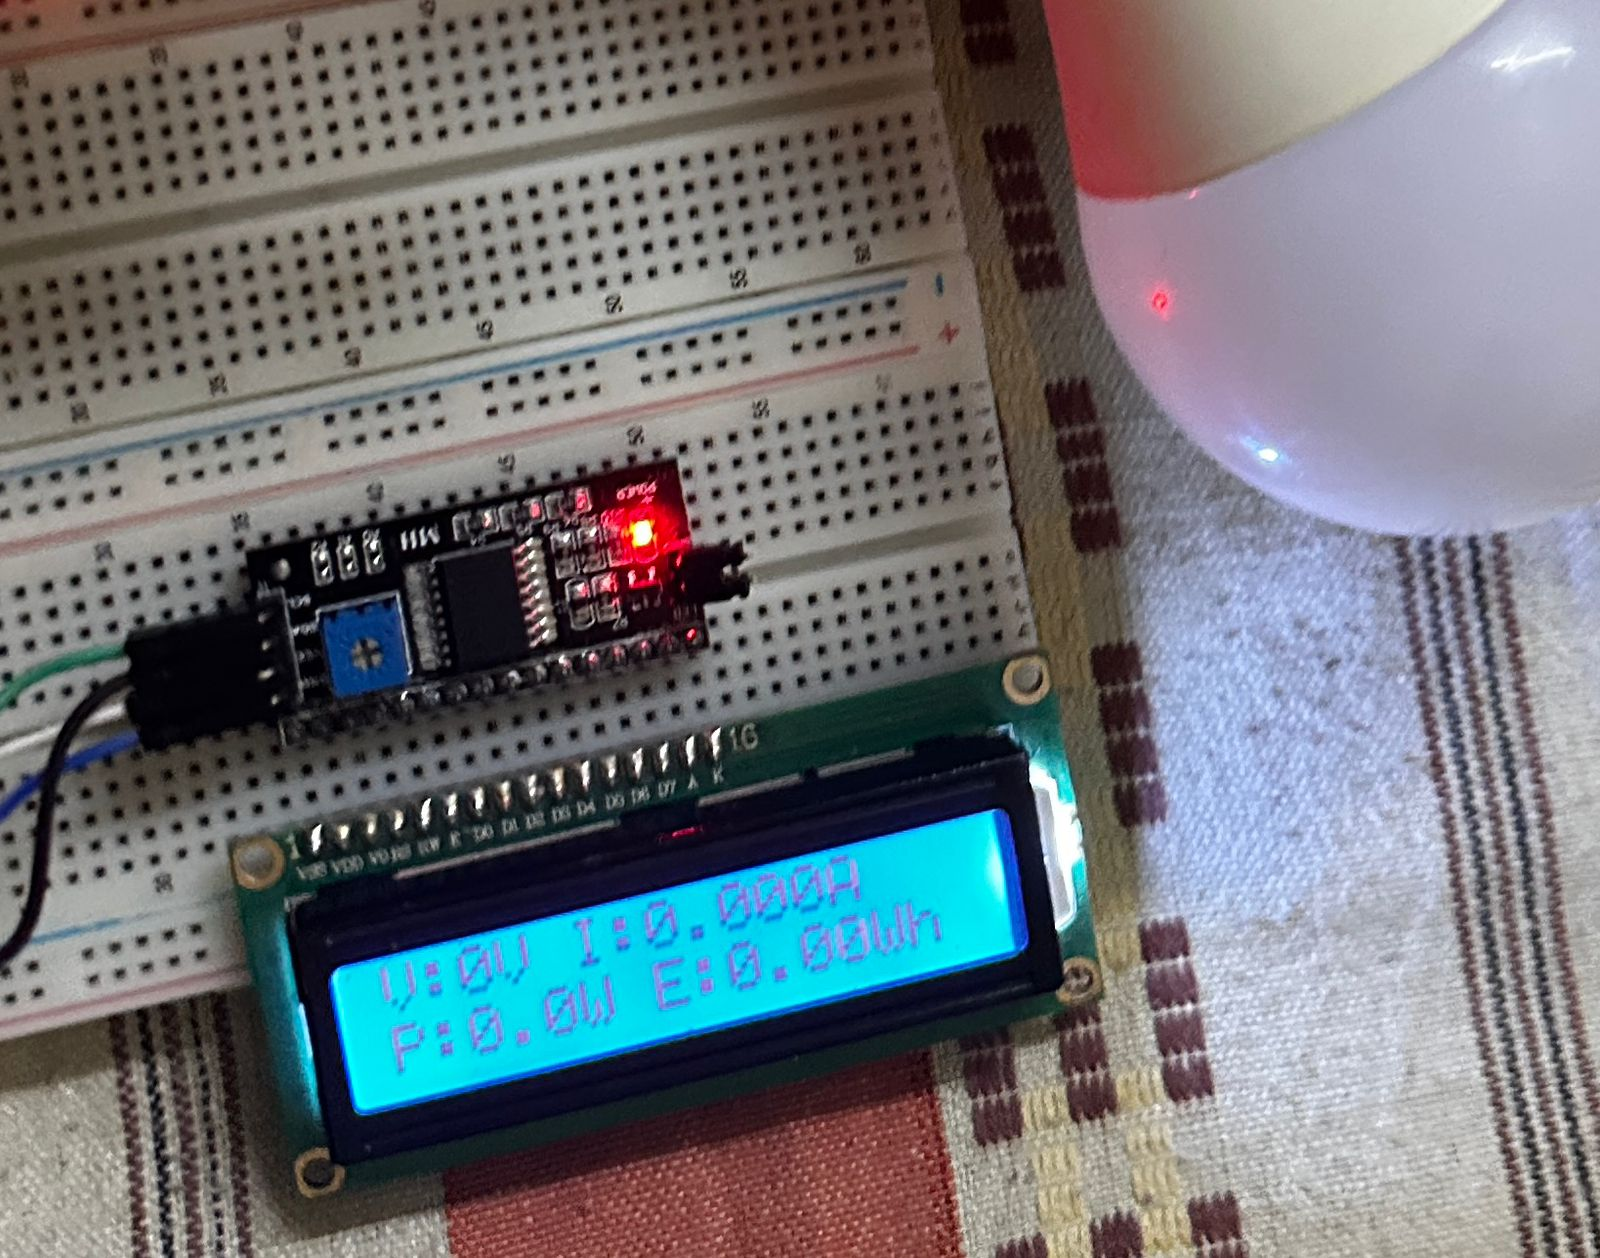
\includegraphics[width=0.9\linewidth]{WhatsApp Image 2024-12-22 at 18.50.10.jpeg}
        \caption{No load is connected}
        \label{fig:No load}
    \end{figure}
    \begin{figure}[H]
        \centering
        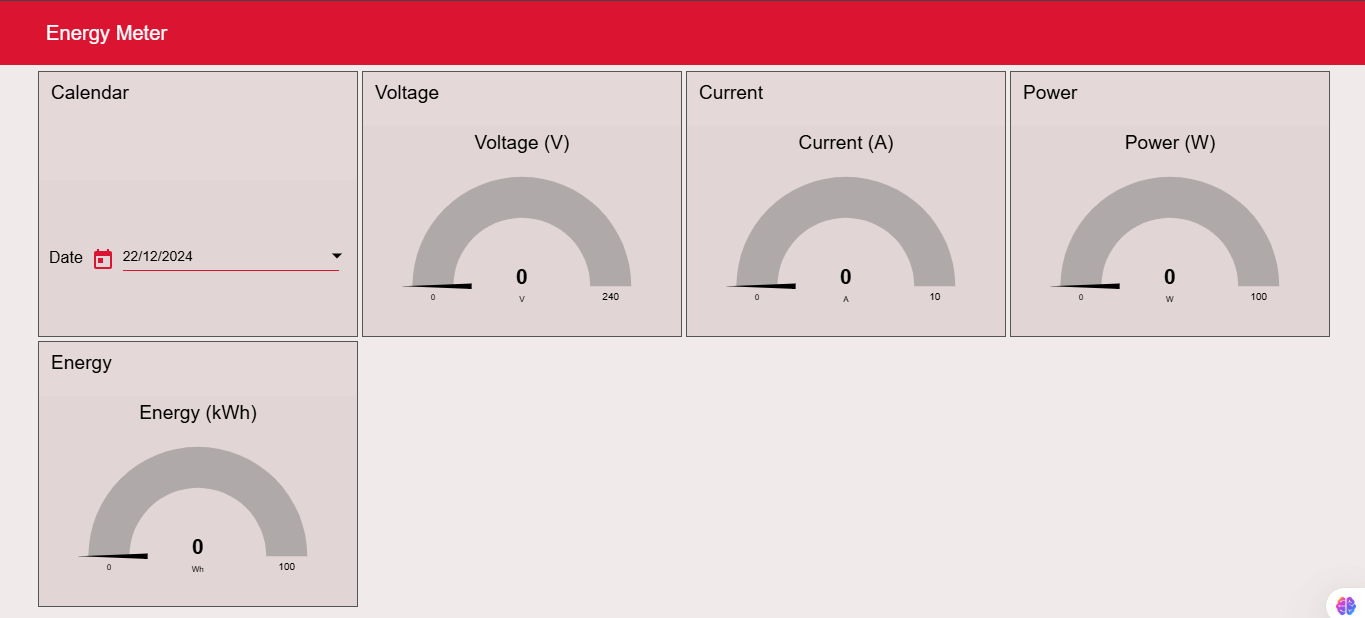
\includegraphics[width=1.0\linewidth]{Project/Screenshot 2024-12-22 162604.png}
        \caption{No load detection on Node-Red}
        \label{fig:No load on Node-red}
    \end{figure}
    \item When a 12W bulb is connected to the sensor
    \begin{figure}[H]
        \centering
        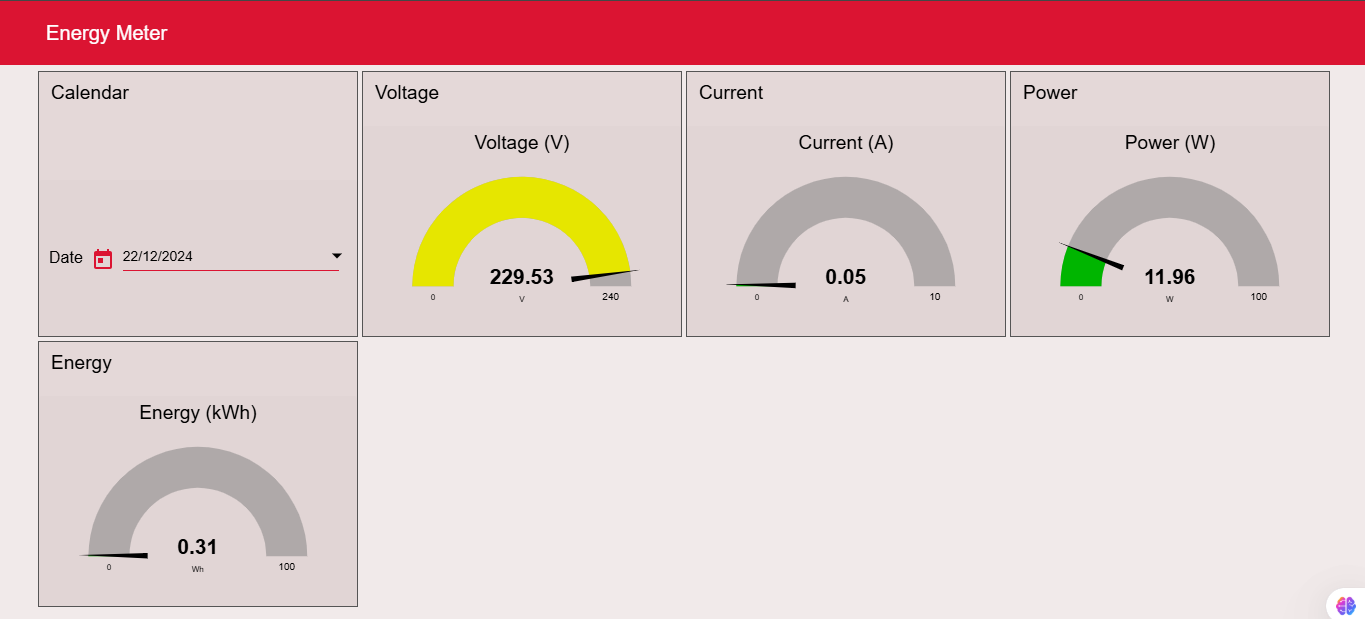
\includegraphics[width=1.0\linewidth]{Project/Screenshot 2024-12-22 163714.png}
        \caption{12W Bulb load readings on Node-red}
        \label{fig:Load on Node-red}
    \end{figure}
\end{itemize}

\subsection{Discussion}
In this project, we utilized a voltage sensor with a measurement range of 0–1000V and a current sensor rated for a maximum current of 5A with a sensitivity of 185mV/A. These sensors provided raw analog data, which was processed by the ESP32 microcontroller’s ADC (Analog-to-Digital Converter). However, the journey from raw data to accurate energy readings involved several challenges and learning experiences.
\subsubsection{Calibration Challenges and Solutions}
One of the primary challenges we faced was ensuring the accuracy of sensor readings. The sensors initially provided raw output data that did not directly correspond to the actual voltage and current values. Calibration was essential to establish a linear relationship between the sensor output and the real-world measurements.
\begin{itemize}
    \item \textbf{Voltage Sensor Calibration:} The voltage sensor required a scaling factor to translate its output into accurate voltage readings. We applied a series of test voltages and measured the corresponding sensor outputs to determine the scaling factor.
    \item \textbf{Current Sensor Calibration:} For the current sensor, the sensitivity of 185mV/A was utilized to calculate the current based on the sensor's voltage output. We tested the sensor with known loads to verify and refine the calculations.\
    \item \textbf{Handling ADC Non-Linearity:} The ADC of the ESP32 introduced slight non-linearity and noise, which affected the precision of readings. We mitigated this by averaging multiple samples for each measurement, reducing the impact of noise and ensuring consistent accuracy.
\end{itemize}
\subsubsection{Hardware and Software Integration}
This project required seamless integration between hardware and software components. Developing firmware for the ESP32 to handle sensor data acquisition, calibration, and MQTT communication was a critical aspect. Challenges included managing real-time data processing while maintaining system responsiveness.
\vspace{5mm}

Through this project, we gained substantial knowledge about the design and implementation of IoT systems. Specifically, we learned about:
\begin{itemize}
    \item Sensor integration that how to set sensor characteristics and calibration techniques to achieve accurate readings.
    \item Implementing MQTT and creating Node-Red Dashboard for real-time data transmission and handling potential connectivity challenges.
    \item  Overcoming challenges in calibration, connectivity, and hardware-software integration strengthened our practical skills.
    \item Gaining insights into power and energy measurement concepts and their application in real-world scenarios.
\end{itemize} 

This project not only improved our technical expertise but also enhanced our understanding of IoT applications, paving the way for future advancements in energy monitoring and smart devices.

\section{Conclusion}
   In this project,  the IoT-based smart energy meter successfully monitored voltage, current, power, and energy consumption with high accuracy in real-time. By addressing challenges in sensor calibration, ADC noise, and MQTT connectivity, we achieved reliable data acquisition and seamless remote monitoring on desktop and mobile. This project enhanced our understanding of sensor integration, IoT communication, and microcontroller programming. The experience gained in tackling hardware-software challenges and ensuring system accuracy has been invaluable. This project not only met its objectives but also provided a strong foundation for future innovations in energy monitoring and IoT systems.








\end{document}
 

